% !TeX root = ../main.tex

\chapter{引言}
\label{cha:intro}

\section{研究背景}
近些年来,机器人研究的方向逐渐从大型机械、传统制造转向小型化、快速制造、精细控制、人机交互等方面,仿生设计也始终是热门关注点。传统的轮式机器人已经比较成熟,而不能满足复杂地形的需要,因此足式机器人引发了许多研究者的关注。这方面进展最快的莫过于四足机器人,上至波士顿动力的Spot机器狗\cite{Spot},下至斯坦福本科生开发的低成本开源四足机器人Doggo\cite{Doggo},大有全民机器狗之势。而其他形式的仿生机器人研究也并未式微,如普渡大学的机器蜂鸟\cite{Hummingbird},斯坦福的单足跳跃机器人Salto-1P\cite{Salto1P},都是小型机器人的优秀代表,后者更是亮相ICRA 2019,与众多机器狗同台竞技,业内人称“蒙特利尔动物园”。

\section{相关研究}
\label{sec:first}
\subsection{Salto}
本项目的直接灵感来自于Salto-1P。Salto-1P是来自加州大学伯克利分校仿生微系统实验室的跳跃机器人。
\begin{figure}[H]
  \centering
  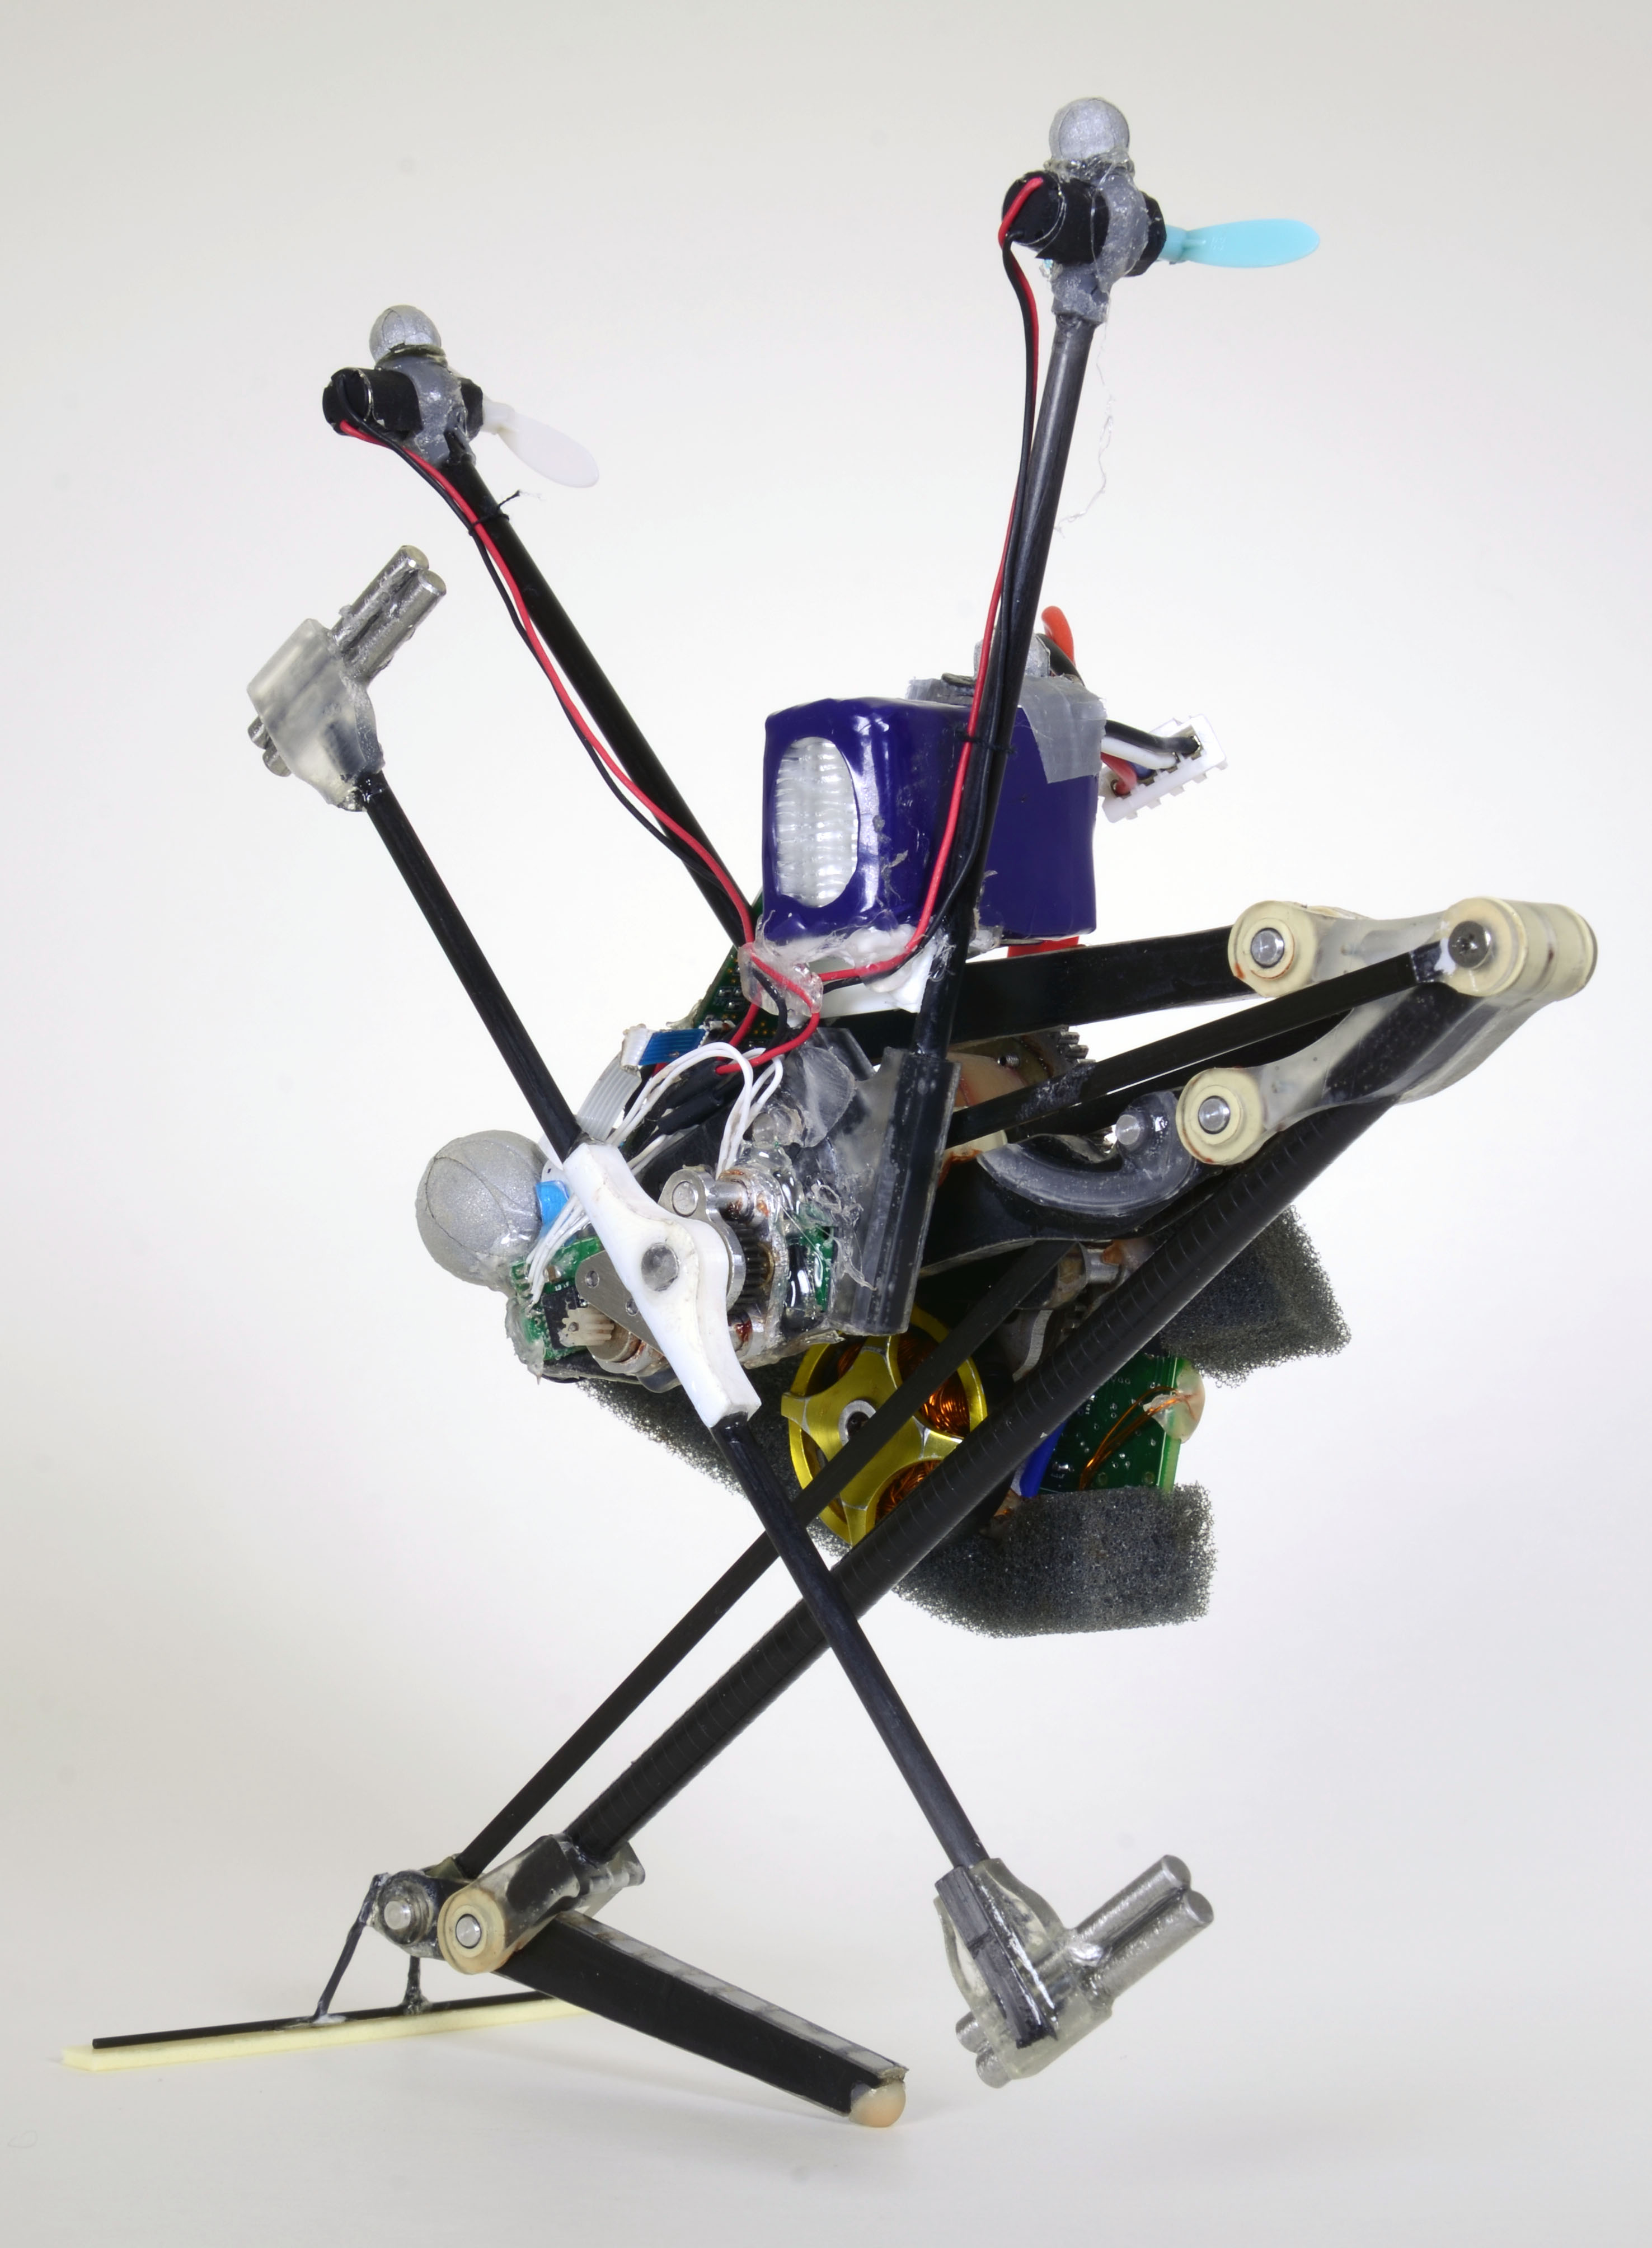
\includegraphics[height=8cm]{Salto-1P.jpg}
  \caption{Salto-1P机器人\cite{Salto1P}}
  \label{fig:salto-1p}
\end{figure}
Salto-1P的主要特点是通过SEA驱动结构实现了能量的存储,以保证跳跃瞬间的能量爆发。它可以每0.58秒进行一次高度1m的连续跳跃,这样的敏捷性无疑是惊人的。初代Salto\cite{Salto}腿长约15cm,重约100g,能量密度137W/kg,各方面指标已经接近或超越其设计之初的模仿对象————自然界的夜猴。为了实现精确控制,Salto身上装备了用于控制姿态的尾部,Salto-1P还配备了一对螺旋桨。前者在研究中只进行一次跳跃,而后者由于通过两个螺旋桨控制横滚(Roll)和偏航(Yaw),再加上尾部对俯仰(Pitch)的控制,实现了对空中身体姿态三个自由度的完全操控,因此可以做到连续跳跃。\\
对本项目的启示:
\begin{itemize}
  \item 本项目的弹跳部分设计参照了Salto腿部的机械模式,以提供有利于弹跳的机械增益曲线。
\end{itemize}
\subsection{Multimo-bat}
Multimo-bat多模态蝙蝠机器人是CMU机械系一位博士生2014年的作品。  
\begin{figure}[H]
  \centering
  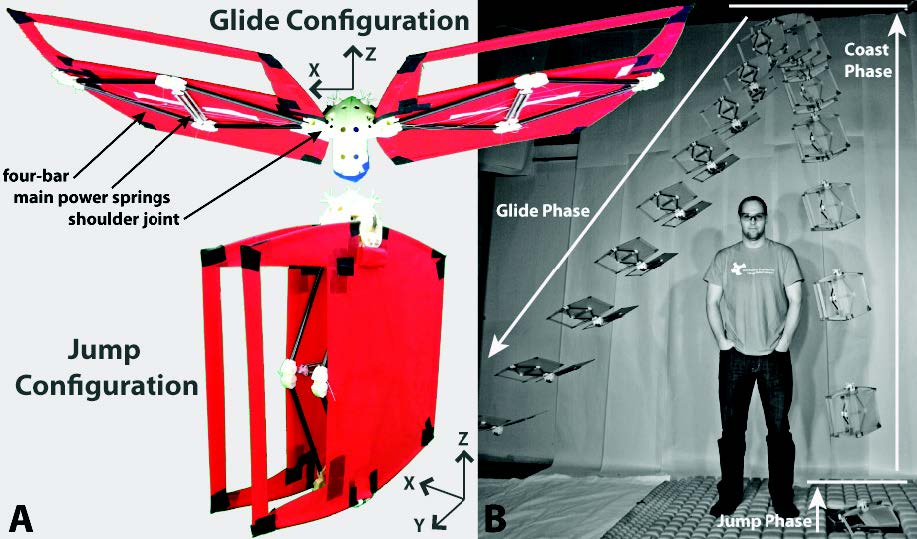
\includegraphics[height=8cm]{Multimo-bat.jpg}
  \caption{Multimo-bat机器人\cite{multimo}}
  \label{fig:multimo}
\end{figure}
如图\ref{fig:multimo}所示,该机器人主要拥有两个形态:跳跃态和滑翔态。其主要结构由身体和四连杆可折叠机翼构成。一个完整的跳跃滑翔运动过程如下:
\begin{enumerate}
  \item 图\ref{fig:multimo_struct}(a)中的主电机转动带动图中白线拉紧,此时四连杆收缩,电能转化为翼上弹簧的弹性势能存储起来。当收紧到一定程度后,触发内部结构的离合装置,充能完毕。
  \item 图\ref{fig:multimo_struct}(b)中的SMA丝通电发热收缩拉动离合器解锁,机翼快速弹回原位,弹簧释放能量,机器人跳起。
  \item 当机器人跳至最高点时,张开机翼,进入无动力滑翔模式。
\end{enumerate}
对本项目的启示:
\begin{itemize}
  \item 该项目的整体功能与本项目目标基本相同,其滑翔模式下通过控制重心来调整机翼攻角而不增加自由度的思想可以简化系统设计,增加鲁棒性。
\end{itemize}
\begin{figure}[h]
  \centering%
  \begin{subfigure}{3cm}
    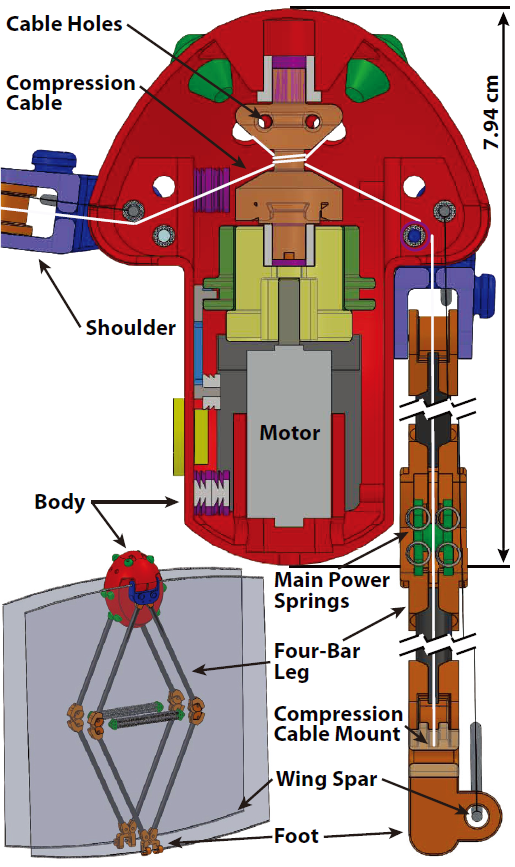
\includegraphics[height=10cm]{Multimo-bat_Structure.png}
    \caption{整体结构}
  \end{subfigure}%
  \hspace{10em}%
  \begin{subfigure}{0.5\textwidth}
    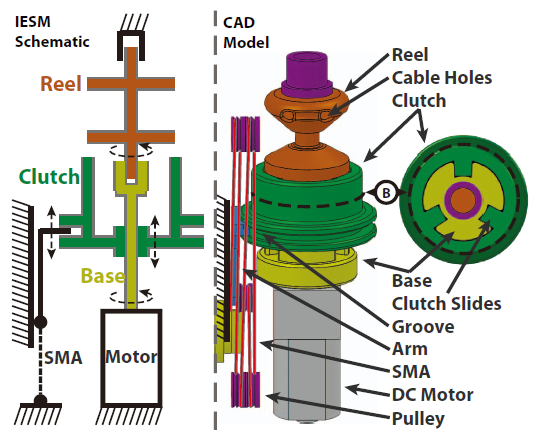
\includegraphics[height=8cm]{Multimo-bat_Structure2.png}
    \caption{离合器}
  \end{subfigure}
  \caption{Multimo-bat主要结构\cite{multimo}}
  \label{fig:multimo_struct}
\end{figure}

\subsection{EPFL Jumpglider}


对本文的启示:
\begin{itemize}
  \item 给出了跳跃滑翔模型的理论基础,以及最优化滑翔距离的方式。
\end{itemize}